\section{Literature review}

The world's population is growing rapidly.  It reached 6 billion people in 1999 and is anticipated to reach 8.1 billion in 2025 and 9.6 billion in 2050 \citep{Alexandratos_2012_World}.  Our long-term ability to meet growing needs for food seems uncertain.  Thus, one of the greatest challenges is increasing food production in a sustainable way so that everyone can have adequate food and proper nutrition without over-exploiting the Earth's ecosystems. 

Rice is predominantly produced in Asia, so much so that thirty--one percent of the rice harvested globally comes from Southeast Asia alone \citep{OECD_2012_Agricultural}. The highest levels of productivity are found in irrigated areas, the most intensified rice production systems. Farmers can grow more than one rice crop per year here. Approximately 45 percent of the rice growing country in Southeast Asia is irrigated, with the largest irrigated areas been found in Indonesia, Vietnam, Philippines and Thailand \citep{Mutert_2002_Developments}. In South Asia, the two major rice-growing countries are India and Bangladesh. India has the largest rice growing area globally, about 43 million hectares, and contributes 25 percent of global rice production. Combined, rice production in South and Southeast Asia contributes around half of global rice production. If rice production in South and Southeast Asia is threatened, it will significantly affect global rice production.

Pests in rice production are significant yield reducing factors globally. \cite{Oerke_2005_Crop} estimated that weeds, animal pests, and disease caused losses around 10.2, 15.1 and 12.2 percent of global rice production, respectively. In most Asian countries, rice yields average 3-5 t/ha.  One recent survey estimated that between 120 and 200 million tons of grain are lost yearly to insects, diseases, and weeds in rice fields in tropical Asia \citep{Willocquet_2004_Research}. The mean region-wide rice yield loss due to pests was estimated at 37 percent \citep{Savary_2000_Quantification}.

In crop fields, pests or so-called biotic constraints can be defined as organisms that cause plant injuries and lead potentially to economic losses. Among the pests that attack rice are microorganisms (viruses, mycoplasmas, phytoplasmas, bacteria, oomycetes, and fungi) that can cause diseases, parasitic plants, weeds, invertebrates (insects, mollusks), and even vertebrates such as rats and birds can cause serious damages.

\subsection*{Rice Pests}

Rice fields are human-managed ecosystems, which harbor diverse communities of plant, animal, and microbial species. Many of them indeed benefit with rice plants, such as predators, parasitoids, flowering plants, and soil bacteria \citep{norton2010rice}. However, there are some species threatening the rice plant's health and can cause the quantity and quality losses. I briefly review some pests including weeds, animal pests, and diseases that are concerned the major rice production.

%Within the literature review part, I summarized major rice pests including weeds, animal pests and diseases from several scientifically reliable sources such as websites (\citet{irrirkb}), books (\citet{ouricedisease} and \citet{mew2002handbook}), and articles.

\textbf{Weeds} are plants considered as unwanted plants in the crop growing area and compete for nutrition, water, or light with cultivated crops.  Weeds are the cause of severe yield reduction problems. In Asia, they are estimated to cause yield losses up to 80 percent, depending on rice field conditions (crop establishment, water management, field management). Weeds also reduce grain quality, and increase the production costs such as labor cost and input costs \citep{litsinger1991crop}.

\textbf{Rat} causes serious yield reduction problems in many countries in Asia such as Bangladesh, Cambodia, People's Republic of China, India, Indonesia, Lao People's Democratic Republic, Malaysia, Myanmar, Philippines, Thailand, and Vietnam. \textit{Rattus argentiventer} is the major rat pest species in Southeast Asia.  Crop losses due to this species are typically about 10 to 20 percent. Rat damage in the rice fields is easily observed when a large number of the tillers are cut. They damage to rice plants at all stages from sowing to storage. At the seedling stage, they chop down the young seedlings and also feed on the endosperm \citep{singleton2003impacts}. 

\textbf{Golden apple snail} (\textit{Pomacea canaliculata} (Lamarck)) is an exotic species in Asia. Its origin is South America. They were introduced to farmers in countries in Asia to increase their income and as a source of protein in their diet, and also as an aquarium pet \citep{joshi2007problems}.  Now they are spreading around Asia and have become a major rice pest in the areas where they have founded. Snails attack younger seedlings at deep water levels. \citep{basilio1991problems} estimated that snail density at 8 snails/square meter could damage the rice seedlings up to 93 percent. However, seedlings become tolerant to snail attacks at the age of 40 days old \citep{sin2003damage}.  

\paragraph{Insect pests} are serious threats to rice production in nearly all regions, where rice is grown. Yield losses due to insect pests based on surveys from 11 countries were estimated at 18.5 percent \citep{pathak1994insect}.  The introduction of high yielding technology in the 1960s involving rice varieties with high tillering ability, denser plant spacing, high fertilizer application and irrigation where farmers planted two or three crops per year provided abundant habitat and food sources where the insect pests can reproduce continuously throughout the year. Moreover, the use of nitrogen fertilizers increased the insects' reproductive potential \citep{bottrell2012resurrecting}. In South and South East Asia, rice is grown in warm, humid environments conducive to the survival and proliferation of key insect pests: stem borers, rice loaders, brown planthoppers, whitebacked planthoppers and green leafhoppers.


\textbf{Stem borers} are ubiquitous throughout rice fields in Asia and cause some damage in every rice field every year. There are six species, but rice yellow stem borer, \textit{Scirpophaga incertulas} (Walker), is the most destructive species in Asia, which may cause 20 percent yield loss in early planted rice crops, and 80 percent in late-planted crops. The larvae bore into the stems and eat their way down to the base of the plant hollowing out the stem. If the damage occurred during the vegetative stage the central leafs do not unfold, turn browns and die off, this is called ``deadheart''. If this damage occurs during the reproductive stage it results in the drying of the panicles, which may not emerge or do not produce grains. This is called ``whitehead''. Yield losses from stem borer damage can reach up to 95 percent in severe infestations. \todo{Citation needed, you claim that YSB is the most destructive.}

% what it tiller mortality?
\textbf{Asian rice gall midges}, \textit{Orseolia oryzae} (Wood-Mason) damaged tillers are characterized by pale green color and the stems elongated and converted into hollow tub called ``onion leaf'' or ``silver shoot''\citep{pathak1994insect}. The Asian gall midge could cause significant yield losses of US \$ 80 million annually in India \citep{bennett2004new}. 

\textbf{Rice leaf feeders}, which include: rice leaffolder (\textit{Cnaphalocrocis medinalis}), rice whorl maggot (\textit{Hydrellia philippina} Ferinoand), rice hispa (\textit{Dicladispa viridicyanea}) (Kraatz), and  rice thrips \textit{Stenchaetothrips biformis} (Bagnall) often attack rice in the early rice stages, causing highly visible leaf injuries.\todo{citation}  Rice leaffolder larvae fold the leaves by stitching the leaf margins and feed by scraping green leaf tissue Leaves damaged by rice hispa appear irregular translucent white patches paralleling to the leaf veins. Rice leaf miner. Rice thrips are more serious pests in the dry season than wet season. It infests the rice plant during the seedling stage or two weeks after early sowing. Leaves damaged by thrips are curl and discolored. However, the injuries caused by these insect pests are not considered important as often does not translate into a yield loss because of plant compensation \citep{pathak1994insect,shepard1995rice}. \todo{Revise this para for clarity and citations for the pests.}

% revise for clarity
% what about small brown planthopper?
% I think you'd best double check whether these transmit a disease or a virus.
\textbf{Rice sucking insects}: brown planthoppers (BPH), \textit{Nilaparvata lugens} (St\aa l), small brown planthoppers (SBPH), \textit{Laodelphax striatellus} Fall \'en and whitebacked planthoppers (WBPH), \textit{Sogatella furcifera} (Horvath), and rice black bugs are sucking insects that feed on rice plants. As a result of feeding by both nymphs and adults at the base of the tillers, plants turn yellow and dry up, turn brown and die. At early stages of heavy infestation round and yellow, and brownish patches appear due to the drying up of the plants. This condition is called ``hopperburn''. It can cover large patches in rice fields. Moreover, the BPH are the vectors of \textit{Rice Ragged Stunt Virus} and \textit{Rice Grassy Stunt Virus}. The SBPH also transmits rice viral diseases such as \textit{Rice stripe virus} and \textit{Rice black-streaked dwarf virus}, The green leafhoppers, \textit{Nephotettix malayanus} and \textit{Nephotettix virescens}, can transmit rice viruses such as Rice tungro virus, Rice yellow dwarf, yellow-orange leaf, transitory yellowing \citep{ling1972rice}. Rice black bugs belong to several species, but Malaysian black bug \textit{Scotinophara coarctata} is the most common in Asia. They feed on the rice plant from seedling to maturity growth stages. Their damage can cause reddish brown or yellowing of plants. Leaves also have chlorotic lesions. Severe damage may show the symptom called ``bugburn'' showing wilting of tillers with no visible honeydew deposits or sooty molds. Plants are also stunted; and can develop stunted panicles, no panicles, incompletely excerted panicles, and unfilled spikelets or whiteheads at booting stage \citep{shepard1995rice}. \todo{Citations needed for plant hoppers and vectoring. Watch your terminology. I've already warned, you interchange the pathogen with the disease too much. Also check viral naming conventions for proper capitalization and italics.}

\textbf{Grain sucking insects} include rice bugs or slander rice bugs, and stink bug. The common species of them are \textit{Leptocorisa oratorius} F.\todo{F. what?} and \textit{Leptocorisa acuta Thunberg}. They are found commonly at the flowering to milk stages in all rice environments. They insert their needlelike mouthparts into the grains. Damaged Rice grains by these insects are characterized by deformed, spotty and empty grains. They are reported that can cause yield loss up to 30 percent. There are many rice stink bugs species reported that they damage rice grains, but the most common stink bug is \textit{Nezara viridula} (Linnaeus). They penetrate the grain hull with their strong mouthparts to feed on the endosperm \citep{shepard1995rice}. \todo{Revise this para for clarity and capitalization.}


\paragraph{Rice diseases} result in yield reductions of 10 - 15 percent in tropical Asia \citep{willocquet2004research}. Sheath blight and brown spot are important diseases in rice in Asia, each responsible for 6 percent of yield losses, whereas rice blast, bacterial leaf blight account for 1 - 3 percent and 0.1 percent of yield losses, respectively. Sheath rot, stem rot, and those known as sheath rot complex and grain discoloration are responsible for rice yield losses ranging from 0.1 - 0.5 percent, respectively. All other diseases alone or in combination do not cause more than 0.5 - 1 percent of yield losses based on estimates \citep{Savary:2000vr,mew2002handbook}. I briefly review some rice diseases that are commonly found in South and South East Asia. 

\paragraph{Foliar diseases} include brown spot, rice blast, narrow brown spot, bacterial leaf blight, bacterial leaf streak, \textit{etc}.

\textbf{Brown spot}, caused by \textit{Cochliobolus miyabeanus} (Ito \& Kuribayashi) Drechs. ex Dastur (anamorph: \textit{Bipolaris oryzae} (Breda de Haan) Shoemaker) is one of the most important disease of rice in Asia and is reported across South and South-East Asian countries. The disease appears as small oval or circular, dark brown spots on leaves or glumes. The disease is seed-transmitted and infected seed is the primary inoculum source. The disease develops quickly in fields with scarce water supply and nutritional imbalance, particularly low nitrogen, phosphorus and potassium \citep{barnwal2013review}.\todo{Yield losses?}

\textbf{Rice blast}, caused by \textit{Pyricularia grisea} Sacc., synonym \textit{P. oryzae} Cavara (teleomorph: \textit{Magnaporthe grisea} (Hebert) Barr) \citep{rossman1990pyricularia}\todo{Use teleomorph first, then anamorph as it's deprecated}, overwinters in rice straw and stubble and spreads rapidly by airborne spores. The symptoms can be found on all part of the plant including leaves, leaf collars, necks, panicles, pedicels, roots, and seeds. Leaf blast symptoms are characterized by elliptical or spindle shaped lesion with whitish-gray or greenish center and brown or purple margins with yellow halo. Neck or panicle blast, which is more damaging, appear as a dark necrotic lesion covering partially or complete around the panicle base or secondary branches. It may lead to breaking of panicles resulting in few or no grain setting. Disease is favored by high nitrogen. Soils with poor silica availability are blast conducive. Blast is highly destructive in lowland rice in temperate and subtropical Asia, and upland rice in tropical Asia, Latin America and Africa \citep{ouricedisease}.

\textbf{Narrow Brown Spot}, caused by the fungus \textit{Cercospora janseana} (Racib.) O. Const., synonym:\textit{C. oryzae} Miyake (teleomorph: \textit{Sphaerulina oryzina} K. Hara), \todo{Again, teleomorph first, then anamorph} characterized by small, narrow, elongated dark brown spots spreading uniformly over the leaf. Symptoms are usually extensive during the later stages of growth, with lesions appearing just prior to anthesis. Severe damage decreases the grain quality and reduces the milling recovery, but has no significant effect on yield losses. \todo{Citation}

\textbf{Bacterial leaf blight} or bacterial blight, caused by \textit{Xanthomonas oryzae} pv. \textit{oryzae} (Ishiyama) Swings \textit{et al.} (synonym: \textit{X. campestris} pv. \textit{oryzae} (Ishiyama) Dye is characterized by yellowing and dry leaves. The disease developed at the tips of the leaf and spread down one or both sides of the leaf and maybe through the middle leaf. The disease occurs in both tropical and temperate environments, particularly in irrigated and rainfed lowland areas. The high wind and rain were believed to aid in rapid dispersal of the pathogen. In severe epidemics, yield losses can range from 20 - 40 percent \citep{sonti1998bacterial}.

\textbf{Bacterial leaf streak}, caused by \textit{Xanthomonas oryzae} pv. \textit{oryzicola} (Ishiyama) Swings \textit{et al.} is characterized by fine translucent streak between veins. Then the streaks become yellowish-gray, the lesions coalesce, then eventually turn to brown to greyish white causing the leaves to die. This disease is common in South and South-East Asia. Severe infection results in poor grain development, broken rice and deterioration in chemical and nutritional composition. \todo{Citation}

\paragraph{Diseases on the tiller} include sheath blight and bakanae \todo{Incomplete}

\textbf{Sheath blight}, caused by \textit{Thanatephorus cucumeris} (A.B. Frank) Donk (anamorph: \textit{Rhizoctonia solani} K\"uhn) is characterized by irregular lesions usually found on the leaf sheaths (initially water-soaked to greenish gray and later becoming grayish white with a brown margin). Sclerotia (small brown-to-black, rocklike reproductive structures) may be present on the stems. Symptoms are usually observed from tillering to milk stage in a rice crop. This fungus lives in the soil and floats to the top when fields are flooded, contacts rice plants and spreads to adjacent plants. Spread of sheath blight is thus favored by dense crop canopies. It occurs throughout the rice growing areas. Sheath blight causes a yield loss of 6\% \todo{Be consistent are you spelling out or using the symbol?} across lowland rice fields in tropical Asia \cite{Savary:2006to}\todo{Why is this citation not in ()?}.

\textbf{Bakanae} or \textbf{foot rot}, caused by \textit{Gibberella fujikuroi (Sawada)} (anamorph: \textit{Fusarium moniliforme} J. Sheld) is commonly found throughout the whole rice growth stages. \todo{Common throughout all rice stages?} Infected seedlings elongate abnormally, becomes slender and the leaves turn pale yellow green. Infected plants develop roots at the upper nodes and the whole plant turns yellow. At booting stage, some infected plants die. This disease was reported that it can cause yield loss up to 20 percent in outbreak areas.\todo{Citation and revise for clarity}

\paragraph{Panicle diseases} commonly include sheath rot, dirty panicle complex or grain discoloration, and false smut.

\textbf{Sheath rot}, caused by \textit{Sarocladium oryzae} (Sawada) W. Gams \& D. Hawksworth (Synonym: \textit{Acrocylindrium oryzae} Sawada), reduces grain yield by retarding or aborting panicle emergence, and producing unfilled seeds and sterile panicles. Sheath rot also reduces grain quality by causing panicles to rot and grains to become discolored. The typical sheath rot lesion starts at the uppermost leaf sheath enclosing the young panicles. It appears oblong or as irregular spot with dark reddish, brown margins, and gray center or brownish gray throughout. \todo{Citation}

\textbf{Dirty panicle} or \textbf{grain discoloration} is characterized by darkening of glumes of spikelets, brown to black, including rotten glumes. This disease caused by multiple fungal species which include, (\textit{Alternaria alternata}, \textit{Altrernaris padwikii}, \textit{Cochilobolus miyabeanus} (synonym: \textit{Bipolaris oryzae}) \textit{Cuvularia} spp., \textit {Fusarium} spp.,\textit{Magnaporthe salvini}, \textit{M. grisea}, \textit{Nigrospora oryzae}, \textit{Sarocladium oryzae}. Affected seeds by theses pathogen have deleterious effects on the quality of seed lots, which indicate to seed health \citep{ouricedisease} and \citep{mew2002handbook}\todo{Clarify last sentence, nonsensical}.
 
\textbf{False smut} caused by \textit{Villosiclava virens} gen. nov., comb. nov. (anamorph: \textit{Ustilaginoidea virens} (Cooke) Takahashi) is characterized by the grain transformed into a mass of spore ball, which is initially orange, then become olive-green, and then greenish black at maturity \citep{tanaka2008villosiclava}. False smut of rice is reported in most rice-growing areas of the worlds. In favorable conditions, which are high humidity, and soils with high nitrogen content, yield loss caused by this disease can reach to 7 - 75 percent \citep{ouricedisease}. \todo{Nothing of mycotoxins?}

\paragraph{Viral diseases} include rice grassy stunt disease, rice ragged stunt disease, and rice tungro disease, \textit{etc}. 

\textbf{Grassy stunt disease}, caused by \textit{Rice grassy stunt virus} is transmitted by brown planthopper. Infected rice plants show stunting and proliferation of short, erect, and narrow leaves that are pale green or pale yellow. The virus reduces yields by inhibiting panicle production. Plants can be infected at all growth stages. They are most vulnerable to infection at the tillering stage. Infected stubble and volunteer rice are sources of rice grassy stunt virus. The virus cannot be transmitted via brown planthopper eggs \citep{ouricedisease,ling1972rice}.

\textbf{Rice ragged stunt disease}, caused by \textit{Rice ragged stunt virus} is transmitted by brown planthopper. Leaves of infected plants have a ragged appearance. Rice ragged stunt virus infection is particularly high in tropical conditions where rice is planted all year around and provides a continuous host for the brown plant hopper vector. Infected stubble and volunteer rice are sources of rice grassy stunt virus. The disease reduces yield by causing partially exerted panicles, unfilled grains and plant density loss. Infected crops will have significant yield losses of up to 80 percent \citep{ling1972rice}.

\textbf{Rice tungro disease}, caused by \textit{Rice tungro spherical virus} and \textit{Rice tungro bacilliform virus}, is transmitted by green leafhoppers. Tungro disease can occur during all growth stages of the rice plant. It is most frequently seen during the vegetative phase. Plants are most vulnerable at tillering stage. It causes leaf discoloration, stunted growth, reduced tiller numbers and sterile or partly filled grains. Tungro is one of the most damaging and destructive diseases of rice in South and Southeast Asia. In severe cases, Tungro susceptible varieties infected at an early growth stage can have as high as 100 percent yield loss \citep{ouricedisease}.

Farmers encountered an estimated average of 37 percent of their yield loss because of pests and disease. This proportion will be reduced when the farmers have efficient pest management. An important concept applied in pest management is ``disease triangle''\todo{Citation}, which explains that an occurrence of plant disease epidemic need three components, virulent pest, susceptible plant and conducive environment. At the farm level, we emphasize the interactions at population level. These interactions depend on not only the physical, biological environment but also man-made activities (Fig.\ref{fig:diseasetriangle}). According to \citet{Savary:2006to}, pest management tetrahedral first discussed by \cite{Zadoks:1979ts} consists of four elements, a pest, crop, the environment and human. Human is recognized the important role in agroecosystem and should be considered to sustainable pest management \citep{Zadok1985}. Humans are not limited to farmers, but also included to farmers' communities, social networks, agro-technology suppliers, food-chain stakeholders, research and extension, and policy-makers. \todo{Revise for clarity}



\begin{figure}
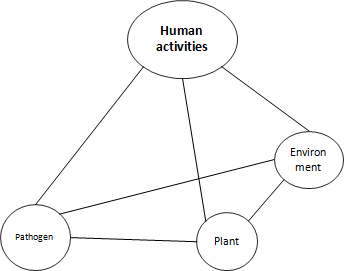
\includegraphics[width=8cm]{distriangle}
\centering
\caption{The epidemiological tetrahedron and the four components of plant disease epidemics: a pathogen; a susceptible host; their environment; and the human activities (e.g., through cropping practices in agroecosystems}.
\label{fig:diseasetriangle}
\end{figure}
<<<<<<< Updated upstream
% Is it not a "competent pathogen", "susceptible host", "conducive environment", and "human activities"?

\section*{The effect of cropping practice on plant pests}
\addcontentsline{toc}{section}{The effect of cropping practice on plant pests}



Each type of pests (animal pest, weeds, pathogens) are \todo{fix this section for clarity and grammar} often coexist and reduce yields in agricultural systems. They may have interactions. In addition to the individual effects on crops, these types of pests and cropping practices can interact and impact crop production. \cite{ouricedisease,ho1994weed,cohen1998importance} and \cite{Mew:2004kh} reviewed the relationships between crop management and pest incidence. 


\subsection*{Crop establishment and pests}
\addcontentsline{toc}{subsection}{Crop establishment and pests}

Crop establishment methods of rice are various, but mainly can be categorized into two types, direct seeding and transplanting. 

<<<<<<< Updated upstream
Weed composition in the rice field is constantly changing. Some weed species are favorably affected by production practice while some are adversely affected. Direct seeded rice more possibly encounters with weed competition than transplanted rice because they emerge simultaneously with rice seedlings and because of the absence of flooding in the early stages. Generally, weeds such as grasses, sedges, and broadleaf weeds are found in direct seeded rice fields, which dominant weeds are \textit{Echinochloa crus-galli}, and \textit{Leptochloa chinensis} among grasses, \textit{Cyperus difformis}, and \textit{Fimbristylis miliacea} among sedges, and \textit{Ammania baccifera}, \textit{Eclipta prostrata}, and \textit{Sphenoclea zeylanica} in the broadleaf category. \todo{Citation}

Compared with transplanted rice, the occurrence of insect pests and diseases is more intense in direct seeded rice because of high plant density and the consequent cooler, more humid, and shadier microclimate inside the canopy\todo{Citation}. The major insect pests of direct seeded rice are brown planthoppers, stem borers, leaffolders, and gall midges. Important diseases that affect direct seeded rice are blast, ragged stunt disease, yellow orange leaf disease, sheath blight, and dirty panicle \citep{pongprasert1995insect}. In addition to insect pests and diseases, other pests that attack emerging rice seedlings are the golden apple snail (\textit{Pomacea canaliculata}) and rats, which are more serious problems in direct seeded rice than transplanted rice.\todo{Citation}


\subsection*{Nutrient management and pest occurrence}
\addcontentsline{toc}{subsection}{Nutrient management and pests}

<<<<<<< Updated upstream
Nutrition management is one of the most important practices of a high production system, but nutrition management will affect the response of rice to pests, as well as development pattern of pest populations due to the change of environments\todo{Change of what environments?}. Soil fertility practices can impact the physiological susceptibility of crop plants to insect pests by either affecting the resistance of individual plant to attack or by weakening plant vulnerability to certain pests. Some studies have also documented how the shift from organic soil management to chemical fertilizers has increased the potential of certain insects and diseases to cause economic losses.\todo{Multiple citations}

Nitrogen, phosphorus and potassium are most often managed by the addition of fertilisers to soils. The others are most often found in sufficient quantities in most soils and no soil amendments are needed to ensure adequate supply unless soil pH limits them. However, I will briefly summarize the effects of nitrogen, phosphorus, and potassium with their relationship to some of the most important rice diseases and insects.

\subsubsection{The effects of nitrogen on pest occurrence}\todo{Occurence or injury or yield losses?}

Nitrogen can prolong the vegetative period and increases the proportion of young to mature tissues in rice plants. It can also reduce the amount of cellulose in plant cell walls, predisposing plants to lodging. Aside from these, increased nitrogen was found to reduce phytoalexins in plant cells. Phytoalexins are anti-microbial compounds that build up in plants as a result of infection or stress, and are associated with resistance to fungal and bacterial diseases. On the other hand, if applied correctly, nitrogen allows better plant compensation and tolerance to injury.\todo{Citation}

Bacterial leaf blight can be aggravated by too much nitrogen, and it is even more problematic during the wet season. This is one reason why the recommendation for nitrogen fertilizer during the wet season is lower compared to the recommendation during the dry season. Other than bacterial leaf blight, excessive nitrogen can also be conducive to the development of many other diseases, such as bakanae, bacterial leaf streak, false smut, leaf blast, sheath blight, and sheath rot.\todo{Citation}

As with the impact of nitrogen on the disease, excessive nitrogen application was force more occurrence of insect pest especially stem borers, whorl maggots, brown planthoppers and leaffolders \citep{chau2003impacts,litsinger2011cultural,rashid2014effect}\todo{Revise for clarity}. The effect of nitrogen on rice insect pests are ambiguous. For example, the number of whorl maggot and rice thrips population were not develop following as the dose of nitrogen increase \citep{chau2003impacts}\todo{Revise for clarity}.

\subsubsection{The effects of phosphorous on pest occurrence}

Just as important as nitrogen, phosphorous is another essential nutrient element that promotes vigorous root development and is responsible for hardening plant tissue. Phosphorus also shortens vegetative period of the plant, as opposed to the effect of nitrogen. Proper timing in the application of phosphorus may lower the incidence of brown spot and leaf blast.\todo{Citation}

In relation to disease incidence, what we know is that phosphorus can reduce the occurrence of bacterial leaf blight and brown spot, but may promote leaf blast and sheath blight of rice. The effect of phosphorus on the population of rice insect pests was not strong \citep{chau2003impacts,rashid2014effect}, but the results of \cite{rashid2014effect} showed that increased phosphorus applicant enhanced the population of brown planthoppers.

\subsubsection{The effects of potassium on pest occurrence}

Among the three essential nutrients mentioned, potassium appeared to be the most consistent and effective in minimizing disease incidence. It was found to lower the infection rate of bacterial leaf blight, leaf blast, and brown spot, sheath blight, sheath rot, stem rot and narrow brown spot\todo{Citation}. This is because K is found to increase the concentration of inhibitory amino acids in the plants as well as phytoalexins\todo{Citation}. Potassium also hardens the plants tissues which can minimize lodging incidence and support faster recovery of injured or stressed plants\todo{Citation}. There were not many studies about the effect of potassium on the rice insect pests. \cite{rashid2014effect} showed the result in Bangladesh that high potassium application decreased population build up and dry weight of brown plant hoppers and \cite{salim2002effects} reported that reported that deficiency of potassium in rice plants increased population build up of white backed planthopper and application of high dose of potassium to rice plants decreased population build up of the insect.

\section*{Interactions between coexisting rice pests}
\addcontentsline{toc}{section}{Interactions between coexisting rice pests}

<<<<<<< Updated upstream
Mixed populations of brown planthoppers and whitebacked planthoppers were reported in many areas. \cite{naganagoud2010studies} reported the experiment multiple pest yield loss to damage function, and economic injury level Iso-loss equation by mutual regression of incidence of two pests. Leaffolder negatively related to stem borers. \cite{selvaraj2012determination} report the population of four major rice insect pests (brown planthoppers, whitebacked planthoppers, stem borers, and leaffolders) by light traps in Tungabhadra area, India from 1988 to 1990. The observations revealed that the mean populations of these pests decreased in 1989 and increased in 1990\todo{Revise para for clarity}.

Many plant diseases are caused by a particular species or even strain in diverse environments. However, there are a number of disease complexes where no one organism causes the full set of symptoms.

Akioshi\todo{check spelling} disease is known as ``hydrogen sulfide toxicity'', causes black crown and root rot, which affect the nutrient absorption. The disease is associated with abnormal soils (silica, potassium, magnesium deficiency). Plants affected by Akiochi become susceptible to \textit{Bipolaris oryzae}, the pathogen of brown spot, which is used as an index of Akiochi \citep{ouricedisease}.

The dirty panicle (grain discoloration) are complex disease caused my many fungal pathogens on the glumes, kernels or both. The fungi that are reported to be associated with discoloration of grains are \textit{Bipolaris oryzae}, \textit{Alternaria padwickii}, \textit{Pyricularia oryzae}, \textit{Fusarium moniliforme}, \textit{F. graminearum}, \textit{Nigrospora oryzae} and \textit{Curvularia} spp.\cite{ouricedisease}. However, it is still conflict such as the Pyriculris test the seed from a filed heavily infested by blast, but no \textit{P. oryzae} isolated\todo{Revise for grammar and clarity}.

The relationships between insect and disease are in the term of vectors\todo{Unclear}. Insects are the vectors of important rice diseases, mostly are viral disease\todo{Revise for grammar}. The incidence of tungro depend on vector population and composition (different species of vector differ in transmission ability, availability of virus source, since the virus is nonpersistence, susceptibility and age of host plant, synchronization of these three factor\todo{Revise for grammar}. Weed hosts of the vectors and of the virus play a role and climates affect all these factors \cite{naganagoud2010studies}. Some found the tungro with yellow dwarf disease \cite{ouricedisease}\todo{Revise for grammar}

\section*{Survey in the field of epidemiological research}\todo{Revise for grammar}
\addcontentsline{toc}{section}{Survey in the field of epidemiological research}\todo{Revise for grammar}

The rice crop system is complex that the number of components is large and their interaction are complex\todo{Revise for grammar}. The dynamic of the system is encompassed by a growing crop, its physical environment, its diseases and pests, and farmers' actions, which influence the whole system. The number of rice pests (diseases, insects, and weeds) to be considered and the levels at which they vary from field to field. A rationale is often deeded to delineate the limits of the system to be addresses\todo{Revise for grammar}.

A survey is a useful tool to provide an adequate account of this diversity and deal with the several pests or variables affecting crop production, which are essential components of systems research in plant protection \citet{Zadoks:1979ts}. Field surveys generate information at the level of the population of crop stands rather than of the individual plot, field, or orchard. Such surveys raise questions regarding variation in injury and its relationships to crop management, crop environment, crop performance, and the occurrence of multiple injuries.


Application of surveys can be found in a huge diversity of research fields, including crop characteristic, cropping practices and single disease or multiple disease and insect. The pest are measurable biological variable that can be used for characterize the injuries profiled (disease and insect injuries syndrome) to stratify farmer's fields account into the characteristic of their production situations.

\cite{savary1995use} emphasized field surveys as the basic means for acquiring information and expanding knowledge to higher scales. Conversely, field surveys and the associated analytical approaches provide a framework in which to characterize disease intensities and their relationships with attributes (including crop management) of the environments where injuries occur; but they usually do not generate crop loss data \textit{per se}.

<<<<<<< Updated upstream
The concept of production situation described the set of factors - physical, biological, and socioeconomic - that determine agricultural production\todo{Citation}. This concept is used here within the restricted scope of an individual rice field and from the limited view point of plant protection. A quick overview of the variables listed in the following survey procedure indicates how this concept is operationalized in a survey: this list includes a few key components of rice crop management (which reflect the physical and socioeconomic environments of a crop and their interactions) and a series of rice pests (that is, insects, pathogens, and weeds).

This approach has the considerable advantage of providing quantitative estimate of the contribution of each constraint to the total yield loss. They study may be considered among the first series, where a set of pest constraints of a crop, simultaneously with environmental variables, and variables representing the current cropping practices were considered. Pests only considered some of the ``yield determining variables''. the approaches may also be considerate an attempt to incorporated the concept of production situation \textit{i.e.} the set of environment that lead to a given yield output of the system\todo{Revise for grammar}. 


\section*{Common techniques for analysis of survey data}
\addcontentsline{toc}{section}{Common techniques for analysis of survey data}

<<<<<<< Updated upstream
Methodologies used to interpret the survey data are developed for studies of the relationships for injuries - yield losses. The development of theses studied started focusing on single-disease (pest) pathosystem to more complex. The classic analytical approaches aim to assess group-wise differences, either in a univariate \textit{i.e.} parameter-by-parameter fashion or using multivariate techniques (\textit{e.g.} multivariate analysis of variance (MANOVA), correspondence analysis (CA), multiple correspondence analysis (MCA), or principle component analysis (PCA)). Univariate methodologies are frequently used to reduce a possibly large number of measured analyses to only those that show the strongest response under the investigated conditions. Examples for such univariate approaches are significance testing methods and simple linear regression model. However, univariate methods fail to apply to different production situation or the scope that model can be applied.


Therefore, multivariate analysis methods seek to capture not only changes of a single pest. Probably the most prominent multivariate analysis techniques applied in the field of survey data are principal component analysis, cluster analysis and correspondence analysis. These analyses do not always; and to yield loss estimate\todo{Revise for clarity}. They can inform us the close relationship between changing production situations and shift crop health syndromes (changes in the dynamics of group disease or crop-limiting factors in an area)\todo{Revise for clarity}. 

Farmers' fields survey datasets are of immense value to plant pathologists; they, however, are generally heterogeneous in format (being qualitative or quantitative) and/or precision. A number of methods, some now old and seldom used, and other more recent and comparatively easier to use, are available to process this type of information. The approached used to analyst these data included three main steps: cluster analysis, multiple correspondence analysis and logistic regression.


Cluster analysis represents another unsupervised multivariate technique suitable for the analysis of survey data with hierarchical cluster analysis and $k$-means clustering being the most prominent representatives. In general, clustering methods group and visualize samples according to intrinsic similarities in their measurements, irrespective of sample groupings. 

%========Network review part============

% why only review empirical works? are all examples here empirical?
The applications of network analysis have increased exponentially over the past two decades in various disciplines. Even though documented applications of network analysis in plant pathology are still relatively sparse, network applications in the social sciences, systems biology and ecology have been increasingly found. Here I review the empirical works that exist and argue that network analysis is a promising approach for exploring questions in the context of plant pathology.

%Network analysis provides fruitful tools for visualizing, analyzing and understanding complex relationships in the studies of plant disease. For instance, network models of genes or proteins pertaining plant defense mechanisms and network models revealing spatial distribution of plant disease through trade networks were already reviewed by \citet{windram2014network} and \citet{Shaw:2014cka}, respectively.


\section*{Network Analysis}
%==========================
\addcontentsline{toc}{section}{Network analysis}
% Good
\subsection*{Introduction to network analysis}
<<<<<<< Updated upstream

Network analysis is used for determining relationships between elements of interest. It offers toolkits for visualizing data in a network model and measuring its properties, and network thinking \citep{PROULX:2005hx}. It has been widely used by various branches of science, such as social sciences, ecology, biology, computer science, and many others to study the interactions between elements, \textit{e.g.}, the relationships of students in school \citep{moody2001race}, species in food webs \citep{krause2003compartments}, interactions of genes or proteins in cells \citep{guimera2005functional}, or the connections of computer in the network \citep{pastor2001epidemic,newman2006modularity}.

\citet{newman2003structure} loosely categorized four types of networks based on different complex data. The first category is social network, representing sets or groups of people forming some patterns of contacts or interactions between them such as the patterns of friendship or business relationships. Analyzing the structure of whole social entities gives us the perspectives from a social network, which enables us to explain the patterns observed. \citet{moody2001race} analyzed the social behaviors in high school students using social network approaches. \citep{Kasari2011social} applied network analysis to compare the social relationships and friendships between children with and without autism spectrum disorder (ADS). The second type of network is an information network or knowledge network. The classic example of this network is the network of citations between academic papers \citep{newman2003structure}. The articles cited other papers, which have related topics. They formed a citation network that has vertices as articles and direct links as citations. The citation network visualizes the structure and the movement of the information. The third category, technological network, is object connected network, or man-made network which represents a physical connection between objects. This network is mostly applied for illustrating physical structures and systems such as the electrical power grid, the connections of rivers, transport systems, etc. The fourth category of network is a biological network. It represents the biological systems such as genes to genes, genes to protein, protein to protein interactions, which enable biologists understand the connections and interactions between individual constituents including genes, proteins, and metabolites at the level of the cell, tissue and organ to ultimately describe the entire organism system. Biologists use biological networks in various branches of biology at different levels (from a single molecule to an entire organism). For example, \citet{yang2014gene,barabasi2004network} studied in the patterns of gene expression in different conditions and different types of cells (normal cells and cancer cells) in order to characterize the genes that change and do not change following the particular conditions; \citet{freilich2010large} applied a molecular ecological network analysis to study the communities of soil microorganisms. Networks revealed the complex relationships between microbial species in soils and their communities. Moreover, network analysis enables ecologists to understand ecological properties and predict the ecological roles of species in a soil ecosystem. Although the application of each type of network approach varies, all four categories of networks share a common empirical focus on relational structure and a similar set of mathematical analysis. 

Network analysis can be a powerful tool to study plant disease. \citet{Lefebvre:2011fo,Jeger:2007tn} applied network models and concepts to study disease spreads in regional networks of plant nurseries and garden centers of \textit{Phytophthora ramorum}, the oomycete causing Sudden Oak Death in the West Coast of the USA and leaf blight and dieback in many ornamental shrubs both in America and Europe. The result could be applied to design measures to control plant disease epidemic from movement of infected material among plant nurseries. 
\citet{Shaw:2014cka} recently reviewed critically about network analysis to plant disease management (\textit{i.e.}, to design ways to reduce the flow of disease in traded plants, to find the best sites to monitor as warning sites for annually reinvading diseases, to understand the fundamentals of how plant pathogen spreads in different structures of simulated trade network models)\todo{Revise for clarity}. \citet{windram2014network} reviewed the applications of network analysis in molecular plant pathology. Network models were applied to reveal plant defense mechanism during plant-pathogen interactions.

\subsection*{Concepts, principles, and methods of network analysis}

A network represents relationships between of elements of interest, which are defined by links (edges) among nodes (vertices). Nodes can be units of interests or studies, and links represent interactions between nodes. Network analysis aims to identify the patterns of associations among nodes, not only features or attributes of particular nodes.

Network analysis follows three principles. Nodes and their behaviors are mutually dependent, not autonomous; links between nodes can be channels for transmission of both material (\textit{e.g.}, money, disease) and non-material (\textit{e.g.}, information, knowledge, relationship, interaction) and; persistent pattern of association among nodes create structure that can define, enable, or restrict the behavior of a node.

<<<<<<< Updated upstream
Network models have two different structures depending on goals of the representation and analysis \citep{borgatti2013analyzing}. Flow models, commonly named directed graphs, represent the network as a system of pathways along which something move such as transportation networks (\textit{e.g.}, highways, railways, and airlines) or communication networks. Since flow networks show the directions of movement between nodes, thus these networks are interesting to study their behaviors. Analysis of flow networks can identify which nodes are more active or which ones are more important connectors. \citet{Jeger:2007tn,Shaw:2014cka} applied such network models to study plant disease spread. Architectural models, or indirected graphs, are mainly used to determine the structure of the network, seeking to discern whether specific structures lead to similar outcomes or whether nodes in similar network positions behave in similar ways. Ecological applications related to the ecology and spatial structure of ``community'' tend to be organized and analyzed as architectural models. For example, \citet{Faust:2012dk} studied networks of soil microbial interactions. Network models can describe how microbial populations change over time, which will require the use of dynamic models of microbial communities. Beyond these basic principles, network analysis enables the calculation of structural properties of nodes, groups, or the entire network.

\textit{Measuring network properties}

A network is made up of nodes and links from relational data. It is constructed from an adjacency matrix, which is obtained from analysis using metric algebra techniques. The row and column headings for an adjacency matrix are identical, listing the names of the components involved in the network. In the simplest case, the cells of the matrix are coded with ``1'' if a link exists between the node or ``0'' if no edge exists. However, a link can be valued. Value indicates a characteristic of the relationship that the research has quantified. The values may be binary, such as whether two friends recognize each other, or variable strength (\textit{e.g.}, the number of mutual friends between two friends). A network link need not imply positive or cooperative interaction; they can also be a negative or competitive interaction between two individuals. 

The distribution of links in a network suggests two important structural characteristics: centrality (importance) of nodes in the network and division of the network into subgroups. Variants of centrality in a network include degree, closeness, and betweenness. Degree centrality of a node is the sum of the value of the links between that node and every other node in the network. This measure tells us how well-connected a particular node is to the other nodes. Closeness centrality is calculated using the length of the path between a node and every other node. This measure could estimate the time required for information or resources to propagate to a given node in a network. Betweenness centrality corresponds to the number of paths in the network that pass through a particular node, and therefore measures the dependence of a network on a particular node for maintaining connectedness \citep{Toubiana:2013cv}. \citet{Deng:2012do,newman2003structure,Toubiana:2013cv} are recommended references for descriptions of the theory and uses, as well as the formal calculation of these measures.



%==========================
\section*{The unique values of network analysis}
\addcontentsline{toc}{section}{The unique values of network analysis}
%==========================

There are four key points that will help to understand network analysis 1) how it differs from traditional approaches of scientific research; 2) how it relates to those traditional approaches; 3) how networks are constructed, manipulated and measured; and 4) what value network analysis offers beyond traditional approaches.

<<<<<<< Updated upstream
The first point of network analysis is that there are two types of data represented in the network graphs; technical and rational data. The first is data characterizing the actors or variables being studied referring to attributes. Attributes describe characteristics of individual actors or variables, for example their race, income or physical location, and are the primary variables considered in traditional approaches. The second type of data is relational data, that is, data about the relationships between individual nodes. For example, \citet{Lazega} represented the network model of cooperation among lawyers in three law firms, through the exchange of various type of resources among them. This model consisted of over 70 lawyers in three different offices in three different cities. Rational data reflected to resources exchange and additional attribute information were included type of practice, genders, and seniority of each lawyers.

Relationships are also referred to as edges (links) in network analysis. Edges cannot be attributed to any single actor. Rather, edges only exist between nodes. This leads to the second point about network analysis that it requires a different conceptual approach. Because edges only exist between nodes, it is useful to think of edges existing in a separate dimension from nodes, who are connected in physical space. This dimension is sometimes referred to as relational space. To visualize the difference, think of someone far away with whom you correspond regularly, say using a phone, email, or Facebook. Even though the two of you are not physically close, you have a strong relationship. The two of you are distant in physical space but close in relational space. This notion of relational space is in part what means when he refers to the space of flows as something distinct from the space of places \citep{Castells}.

The third point that distinguishes network analysis from other approaches is it involves different methods of analysis. Because traditional research methods consider variable attributes in a wide variety of statistical analyses such as measures of center (\textit{e.g.}, mean, median, etc.) and dispersion (\textit{e.g.}, standard deviation, range, etc.), these methods are sometimes referred to as variable analysis, whereas, network analysis models relational data and to measure various characteristics of network structure. For example, for lawyers data \citep{Lazega}, it is natural to ask to what extend two lawyers that both work with third lawyer are likely to with each other as well. This notion corresponds to the social network concept of transitivity and can be captured numerically through an enumeration of proportion of vertex triples that form triangles, so-called cluster coefficient. 


The idea that network structure may be correlated with variable attributes and behaviors is the fourth point to consider in comparing network analysis to other approaches. In network analysis, the arrangement of the network in relational space is basically correlated with the behavior and attributes of those variables. For example, in the network created by \citet{Lazega} lawyers of the same firm may share similar attributes such as office location or department, and lawyers in similar roles within that network may share similar behaviors. Basically, conventional approaches measure various attributes of variable (nodes in a network) and attempts to discern something about the relationships between actors (edges in a network) based on those attributes. When the network structure is simple and the differences in node attributes are clear, the conventional analytic approach is sufficient. However when relationships are complex or node attributes are more nuanced, clear answers using conventional analysis may prove elusive. As a result, network analysis offers a tool to help researchers visualize the large network and disentangle some of the relational complexities within the network, just as cluster analysis and multivariate analysis for help research disentangle the complex data.

\section*{Networks and Plant Pathology}
\addcontentsline{toc}{section}{Networks and Plant Pathology}

<<<<<<< Updated upstream
=======
%% You've cited Jeger, Lefebvre and Windram 2X each already. That's 2X more than necessary to establish that plant pathologists use this method. The more specific examples are probably fine here though.
>>>>>>> Stashed changes
Recently, a broad expansion of applications of network analysis has occurred across many disciplines. It has been evaluated as a promising tool to study a complex system. Plant pathologists have applied network analysis for their research. \citet{Lefebvre:2011fo,Jeger:2007tn,windram2014network} supported that network analysis can be fruitful models in many applications relevant to plant pathology because of its generality and flexibility. For example, the network of main fresh cut flowers movements among European countries was determined the likelihood of introduction of new pathogens and other organisms associated with plants \citep{eagling2007australian}, and plant-pathogen interaction network models were applied to present plant defense mechanisms \citep{dietz2010hubs}. 

The development of network analysis challenges conventional approaches to uncover rational complexities of plant pathology studies. Two fields of research relevant to plant pathology presented particularly strong growth and proved that network analysis has significant potential to augment traditional analysis methods. The first is plant disease epidemiology, which investigates questions related to plant disease spread. The second is plant molecular biology, which investigates questions related to biological networks.

\subsubsection*{Using Network analysis to understand plant disease spread}
<<<<<<< Updated upstream
\addcontentsline{toc}{subsection}{Using network analysis to understand plant disease spread}

Network analysis challenges conventional approaches of studies in plant disease epidemiology, especially underling the spatiotemporal flow of plants and their pathogens \citep{Moslonka2010}. When plant pathological studies were restricted to a single geographical location, there was a limit to thinking about the connections or relationships between plants or fields in different locations. However, network analysis can enlarge the view of studies and can consider whether or not plant pathogens are moving from one field to others in the regions of interest. For example, networks of plant disease spread in trade networks presented the flows of plant disease from infected units (infected plants or epidemic areas) to susceptible units (susceptible plants or areas).

\textit{\textbf{Network models of epidemic development}}
 
The idea of plant epidemics is that the probability of infection embedded in the connection or the contact patterns between susceptible/infected plants, and it forms as the networks. \citet{pautasso2010number} showed a network model of epidemic development (susceptible-infected-susceptible model) in a directed network. In the network model, vertices were represented plant, and their attributes were presented the infectious status (healthy or infected). The epidemic is started at a single node, then nodes with a connection from the starting infected node will be infected at the next time step with a certain probability of transmission. In turn, already infected nodes will be infected at the next time step depending on their infection status and on a certain probability of persistence. The probability of infection transmission is the same for all connections between infected nodes and susceptible nodes over times. Similarly, the probability of infection persistence is the same for infected nodes in a certain network replicate. For each network structure, the two probabilities of persistence and transmission define an epidemic threshold, which is independent of the starting node of the epidemic. This epidemiological model does not result in either susceptible or infected nodes, as nodes will have a infection status along a continuum. Key quantities for epidemiological dynamics in networks were reviewed in \citet{Lefebvre:2011fo}.

\textit{\textbf{Analysis of plant trade network}}

\textit{Phytophthora ramorum} epidemic networks in the horticultural trade are an example of the application of network models in the study of plant disease spread \citep{harwood2009epidemiological,Moslonka2010}. Simulations of spread of \textit{P. ramorum} in different network structures (random, small--world and scale--free network) were found that epidemic threshold, the boundary between a no epidemic an epidemic outcome, is significantly lower for scale-free network, a network is dominated by a small number of nodes with many connections, compared to local, random and small-world network structure. Modeling suggested that was possible to control an epidemic by changing the structure of network, without having to decrease the probability of infection persistence at a nursery site and/or of transmission between sites. Simulation showed that correlation coefficient between link in and out nodes increased with connectivity level for all the structures investigated and underlined the importance of targeted control towards node with more connections than others. 

%% Fix. "The scenario where there are major nodes which both receive plant material from many production sites and supply many retail sites is the most problematic control of this control s target towards such hubs."
%% No idea what this means. Clarify. " Simulations showed that the number of equilibrium. This correlation increase with connectivity level for all the structures investigated and underlines the importance of targeted control towards node with more connections than others \shortcite{Moslonka2010}."

Regardless of the network structure and connectivity level, epidemic threshold is negatively correlated to the correlation coefficient between link in and out nodes, \citep{Moslonka2008}. In presence of high-connected nodes, the most effective way to control disease spread is to move from two-way to a one-way network. That is move from network where overall there is positive correlation among links-in and -out to one where the correlations are negative. In practice this would mean that a nursery network would be dominated by major node, which receives plant materials from many production sites but supply relatively few retail sites, or by major nodes which received plant materials from a few production sites but supply many retail sites. However, the scenario where there are major nodes which both receive plant material from many production sites and supply many retail sites is the most problematic control. The better way to control should target towards the cluster (group of nodes), not only to high-connected nodes. 

<<<<<<< Updated upstream
The last point, the modeling of disease spread in small-size directed networks showed that increasing the proportion of wholesalers (\textit{i.e.}, traders without a preponderance of incoming or outgoing links) tends to decrease the epidemic threshold in local, random, and small-world network. The opposite result is obtained for the proportions of produces and retails. Scale free networks appear instead to be tolerant to changes in these hierarchical categories as the epidemic threshold in this case is governed by the presence of hub rather than by the features of the majority of nodes in the network \citep{Moslonka2010}.

\textit{\textbf{Network models to design strategies of plant disease management}}

Due to globalization, plant trades among countries are increasing and convenient. They potentially caused risks to plant health when they were not under good control. To control the risks of plant disease epidemic through plant trade, network models were applied to present the flows of trade network of plants and plant products across the world and within countries and to develop strategies of plant disease management \citep{pautasso2015network}. Networks could be found hubs or highly connected nodes, which represented locations or countries where imported and exported plants or plant parts. Hubs or highly connected nodes were targets for control disease flows in the scenarios that network presented because they were considered to the likelihood of pathogens actually infecting along particular links. Strategies for disease management should be designed by focusing on links to and from hubs, nodes which have high degree of connectivity, so that it increases efficiency to control plant pathogen spreads. The strategies may aim to remove them from the network \citep{Jeger:2007tn,Lefebvre:2011fo}. Alternatively, strategies may pay attention on them in order to prevent disease spreads. \citet{Shaw:2014cka} suggested placing quarantine efforts on hubs or on connections between major hubs.

Additionally, \citet{pautasso2008epidemiological} showed the good examples, which are co-occurrence networks of the \textit{Phytophthora ramorum} infected plant genera different environments. The networks may be helpful in identifying host taxa playing an important role in spreading a certain disease in the seminatural environment, in crop plants, and plants in the trade. Combining genetic network analysis and data on trace forward and trace back on movement of plants nursery trade supported to identified confidentially \textit{P. ramorum} migration. From this approach, it was clear that the pathogen was introduced originally from nurseries, which \textit{P. ramorum} populations in nurseries are genetically ancestral to all Californian forest populations.


\subsubsection*{Using Network analysis to understand molecular plant pathology}
\addcontentsline{toc}{subsection}{Using Network analysis to understand molecular plant pathology}

For understanding mechanisms of plant-pathogen interactions, network analysis offers tools to visualize interactions of biological components including genes, proteins, and metabolites, which are related to plant-pathogen interactions. Network concepts enable us to characterize interplay of those components following the properties of network structure. Analyzing structural properties of networks may provide useful clues about the biological functions of individual genes, genes complexes, proteins, protein complexes, pathways they participate in.

\textit{\textbf{Presenting biological data with network model}}

Networks are used in different contexts as ways to represent relationships between entities, such as interactions between genes, proteins or metabolites. \citet{wu2007gene} gave the example of a network model built from gene-for-gene relationships between rice and various avirulence genes of the pathogen \textit{Xanthomonas oryzae} pv. \textit{oryzae} causing bacterial leaf blight of rice. Nodes represented isogenic lines of rice and weighted edges reflected the number of shared genes with high resistance (with respect to avirulence genes) in the two isogenic lines of rice. For a plant breeder, this graph can help in identifying particularly promising genes for developing a disease resistant variety.


\textit{\textbf{Network analysis to study biological systems}}


Network analyses have been applied to visualize the myriad information and analyze the complex relationships\todo{Address my comment that's been here on line 298 for months now}. To better understand the collective impact of genes on complex traits and determine what governs their organization, biologists are most likely to apply gene co-expression networks \citep{usadel2009co}. Co-expression networks most commonly use the Pearson's correlation coefficient to establish linear pairwise correlations between gene pairs in an adjacency matrix. Another associative metric that can be used is the Spearman correlation coefficient, which captures nonlinear correlations between genes to be uncovered \citep{usadel2009co,horvath2011weighted}. Once a co-expression network has been generated, identifying modules by clustering can help extract biological meaning from the network. Uncharacterized genes within such a module can be candidates for participating in the same process. Similarly, genes directly connected to (or co-expressed with) known central regulators of a developmental process are candidates within this co-functional framework.

\citet{Zheng2013} used co-expression network inference to investigate plant immunity system of citrus in response to \textit{Candidatus} Liberibacter asiaticus. Gene coexpression networks based on Pearson's correlation coefficients using four transcriptomic data sets studies of citrus infected by \textit{Candidatus} Liberibacter asiaticus bacterium were constructed. The result showed high degree of preservation of gene co-expression patterns across the networks based on different datasets. The network structures revealed hub genes, which have high connectivity. Highly connected nodes (genes) were closely related to Arabidopsis SYP71 encoding a plant syntaxin which functions as a plasma membrane- associated protein transporter. Furthermore, in the study of \citet{mukhtar2011independently}, plant-pathogen interaction networks revealed the interactions of novel \textit{Arabidopsis} protein-pathogen effectors, provided evidences that pathogen effectors target a limited number of host immune proteins, and demonstrated that effectors from very distantly related pathogens interact with the same host proteins. 

The main use of co-expression networks with large collections of static expression data is gene discovery. However, many biologists have attempted to construct differential networks to measure differences in connectivity patterns from datasets with different conditions or targeted experiments \citep{Toubiana:2013cv}. \citet{Lu:2013hga} constructed networks of soil fungal communities. The fungal networks represented two different conditions; yield-invigorating and yield-debilitating soils under prolonged potato monoculture were compared. The authors discussed in differential network concepts that in healthy network three-eighths of fungal groups and soil organic matters were strongly correlated, and in diseases network two of four groups strongly correlated with soil electrical conductivity (EC) and ammonium nitrogen. Differential network analysis showed that average degrees of nodes belonging to \textit{Sordariales} and \textit{Hypocreales} in healthy network substantially were different in disease network. This indicated that they are key species of ecological communities.

\subsection*{A variety of Network Construction Methods}


Until this section, I gave the general information of network analysis with network concepts, network modeling and inference. Ultimately, most of the systems studied from a network--based perspective are dynamic in nature. This underscores the importance of developing tools to understand the interplay between network structures and dynamic processes. I reviewed three network-based analyses: single network, differential network and dynamic network analysis. These techniques from network science have yielded many biological insights \citep{Idekerdiffnet}.

\textbf{\textit{Single Network Analysis}}

Single-network analysis will be used for analyzing a network based on a single data set. It aims to model patterns of relationships between entities to a network, thereby determining its topological properties such as node degree, degree distribution, average path length, clustering coefficient, modularity index \citep{newman2006modularity} to describe the patterns in the network model. These structural properties offer the potential to explore relationships within complex data sets and identify key factors or clusters.

Correlation based networks are widely used for studying biological networks based on pair--wise correlations between variables. Their edges are obtained using correlation-based measures removing spurious relationships. Correlation based measures include linear based correlation (Pearson's correlation, partial correlation) and rank based correlation (Spearman's correlation, Kendall's correlation). Removal of spurious relationships is particularly important when one attempts to establish causal relationships between entities \citep{Toubiana:2013cv}. A correlation based network allows one to define modules (clusters), intramodular hubs, and network nodes with regard to module membership, to study the relationships between modules, and to compare the network topology of different network. 

\textbf{\textit{Differential Network Analysis}}

Networks can respond differently under various environments or with external signals. They can be simplified by focusing on key components and capture only the essential components differently responding between environments in which they play a key role in the modeled response \citep{Peer:2011jd}. Networks are examined by adding or deleting some variables. This allows predicting interactions or components that change following the changed structure of networks. 

Differential network analysis is applied to identify and describe differences between two networks under different conditions. Differential networks from different data sets with different conditions might display different interactions from the single network based on the whole data set, which are disregarded the conditions. The strongest interactions in differential networks are not necessarily those that are strong in the single network. Conversely, they may be weak or absent in single network. Compared between differential networks under different environment conditions, the differential interactions can be implied that they are a result of response to environmental conditions. Moreover, it can be implied that environments influence on the interaction between pairs of nodes contributing to the differential interactions. 

The objective of differential network analysis is to identify the different interactions, that may reveal when condition has changed. For example, the differential network analysis of gene co--expression networks to understand the differences between human and chimpanzee brain was focused on how expression patterns of genes were different in human and chimpanzee brains. These networks are contrasted to find a) non-preserved modules (group of genes with sharing similar expression profiles and presumably similar functions), b) differentially occurred genes, and c) differentially connected genes. The result showed that 

\textbf{\textit{Dynamic Network}}

Biological systems are highly dynamic. They must continuously respond to external signals or the internal state of the system. The responses can be altered slowly or quickly over time \citep{Peer:2011jd}. Thus, realistically the corresponding biological network models must evolve as well. It seems clear that dynamic networks enable us to see and understand the systems and how their dynamic effects change over time. Some understandings previously have been obtained from studies of dynamics of large networks, for example, gene expression or metabolic fluxes network \citep{Idekerdiffnet}.

The main goal of dynamic network analysis moves away from single network analysis, which characterizes absolute properties of the system. It aims to concentrate on a specific dynamic response. Rather than answer what the key factors in the system, it answers what parts of the system are most affected by perturbation. Most commonly, dynamic networks are applied when the edges among a set of vertices or the sets of vertices itself are changing as a function of time. For example, 







